% !TEX TS-program = XeLaTeX
%!TEX program = xelatex
% JSHESS requires the use of the XeTeX (xelatex) typesetting engine to produce the correct fonts
% Not using XeTeX is not going to break anything, it just means that your compiled article
% may look a little different to what it's meant to.
% XeTeX comes bundled with most LaTeX distributions, so everything will probably work fine...
% Just run xelatex foo.tex (or xetex foo.tex) instead of latex foo.tex (tex foo.tex)
\documentclass[10pt]{article}

% Include the jshess package. It's what formats your article correctly
\usepackage{jshess}
\usepackage{amsmath}
 \usepackage{graphicx}

% The title should be both brief and descriptive. It must clearly communicate the nature of the article.
% Ideally, your title should incorporate a key phrase related to your topic within the first 65 characters.
\title{Land-Sea Breeze Forecast Verification}

% Individual author names must be listed in the following style:
% first name then initials with full stops after each initial then last name, followed by any generational suffix.
% Prefixed and post-nominal professional titles and academic qualifications should not be included.
%
% Author names should be listed one after the other without line breaks and separated by commas,
% with the exception of the last name of a multi-name list, which should be separated by the word "and" without a comma.
%
% Numbers indicating author affiliations (see above) should be included in supertext (use \textsuperscript{}) after each name or after the separating comma, if one is used.
\author{Ewan Short,\textsuperscript{1} Ben Price,\textsuperscript{2} Nicholas Loveday,\textsuperscript{2} Derryn Griffiths,\textsuperscript{3} and Michael Foley\textsuperscript{3}}

% Each affiliation should be as concise as possible and in general should not constitute a complete address,
% rather indicate the primary institution of the author(s) and the city and country that the institution is located in.
%
% Each affiliation should be on its own line.
%
% Affiliations should be preceded by the relevant number in supertext (use \textsuperscript{}) that corresponds with the numbers used in the author line above.
\affiliations{%
\textsuperscript{1} ARC Center of Excellence for Climate Extremes, University of Melbourne, Melbourne, Australia \\% These \\%'s are important
\textsuperscript{2} Bureau of Meteorology, Darwin, Australia\\%
\textsuperscript{3} Bureau of Meteorology, Melbourne, Australia\\%
}

% Corresponding author details
\cauthorname{Ewan Short}
\cauthoraddress{School of Earth Sciences, University of Melbourne, Parkville VIC 3052, Australia}
\cauthoremail{ewan.short@unimelb.edu.au}


%%%%%%%%%%%%%%%%%%%%%%%%%%%%%%%%
% Provenance Information
% Editorial Office Use Only
%
\msreceived{Month Year}
\msaccepted{Month Year}
\volume{Vol.}
\issue{Issue}
\shorttitle{Land-Sea Breeze Forecast Verification}
\copyrightyear{2018}
\copyrightauthor{Short et al} % Don't put a full stop after et al here as it will get added automatically.
\setcounter{page}{1} % Starting page number for the article
\pagenumprefix{} % An optional prefix for page numbers
%
%%%%%%%%%%%%%%%%%%%%%%%%%%%%%%%%

\begin{document} % This is important, but you already knew that
\maketitle

%%%%%%%%%%%%%%%%%%%%%%%%%%%%%%%%%%%%%%%%%%%%%%%%%%%%%%%%%%%%%%%%%%%%%%%%%%%%%%%%%%%%%%%%%%%%%%%%%%%%%%%%%%%%%%%%%%%%%%%%%%%%%%%%%%%%%%%%%%%%%%%%%
% Put your abstract here

\begin{abstract}
\noindent This study presents a methodology for comparing the performance of Australian Bureau of Meteorology forecasts of the land-sea breeze with unedited model guidance products, such as those of the European Center for Medium-Range Weather Forecasting (ECMWF) and the Australian Community Climate and Earth System Simulation (ACCESS). The methodology is applied to 13 major Australian airports. The results indicate that at some airports, human intervention to model guidance products adds value to land-sea breeze forecasts, whereas at other airports it does not.    
\end{abstract}

%%%%%%%%%%%%%%%%%%%%%%%%%%%%%%%%%%%%%%%%%%%%%%%%%%%%%%%%%%%%%%%%%%%%%%%%%%%%%%%%%%%%%%%%%%%%%%%%%%%%%%%%%%%%%%%%%%%%%%%%%%%%%%%%%%%%%%%%%%%%%%%%%
% Start your article

\section{Introduction}\label{introduction}
This report describes a methodology for assessing how well the Australian Bureau of Meteorology's official forecast products capture diurnal (i.e daily) wind processes compared to model guidance products like the Operational Consensus Forecast (OCF), the Australian Community Climate and Earth-System Simulator (ACCESS) model, and the European Center for Medium-Range Weather Forecasting (ECMWF) model. The Bureau's official forecast is typically constructed from a blend of model outputs that are then edited by human forecasters, whereas OCF, ACCESS and ECMWF represent unedited model output. Comparing these products therefore provides insight into the added value provided by human forecasters. The analysis presented here is based purely on accuracy in a physical science sense; the analysis cannot account for the social, political or economic reasons human forecasters may have for over or under forecasting certain events or processes.

The analysis provided in this report was performed with software tools I developed using the Bureau's Jive database and code libraries with the assistance of Ben Price and Nicholas Loveday; the code can be found on the Bureau's Jupyterhub server.\footnote{Contact Ben Price (ben.price@bom.gov.au) or Nicholas Loveday (nicholas.loveday@bom.gov.au) for more information.} The code is completely general - any location and time period can be analysed - but to provide a concrete example this report will present a case study of the Darwin airport station during the dry season months of June, July, August of 2017, and the wet season months of December, January, February of 2017/18. 

\section{Methods} \label{methods}
The problem of assessing how well the Bureau's official forecast captures diurnal wind processes has been approached in the most general way possible. Although close to coastlines the land-sea breeze is generally the dominant diurnal wind process, the overall diurnal signal may include mountain-valley breezes, boundary layer mixing processes, atmospheric tides, and urban heat island circulations. Forecasters typically edit model output to account for \emph{both} unresolved sea-breezes \emph{and} unresolved boundary layer mixing; attempting to focus solely on sea-breezes without examining the entire diurnal cycle may thus risk mistaken conclusions, with the effect of one process mistaken for another.

Diurnal wind signals are therefore analysed for each hour of the day. This is done by taking hourly automatic weather station, official forecast and model wind data and subtracting a twenty hour centred running mean from each data point; this provides a collection of wind \emph{perturbation} datasets.\footnote{Unless otherwise stated all vector operations have their usual cartesian-coordinate, componentwise definitions.} 

Thinking of land-sea breezes in terms of perturbations may require a conceptual shift from the usual operational definitions. A forecaster would likely define a sea-breeze to be a reversal in wind direction from a primarily offshore flow during the night and morning, to an onshore flow in the afternoon and evening. However, even if the wind is offshore the entire day, sea-breeze \emph{perturbations} are generally still detectable as a weakening of the offshore flow throughout the afternoon and evening. 

The methods developed in this report can be readily extended to analyse \emph{just} the sea-breezes satisfying the operational definition above. For instance, to study the sea-breezes at a station near a coastline with inward pointing normal vector $\widehat{\boldsymbol{n}}$, the wind perturbation datasets could be restricted to just those days where the corresponding raw wind vector $\boldsymbol{u}$ satisfies 
\begin{equation}
\widehat{\boldsymbol{n}} \cdot \boldsymbol{u} > 0
\end{equation}
for at least one of the hours of that day.\footnote{This and similar techniques could easily be implemented in the existing Jupyter notebook using boolean masking.}

Two closely related indices for assessing the performance of official forecast wind perturbations against those of an unedited model guidance product have been developed; these are outlined below. 

\subsection{The Wind Perturbation Index}\label{daily-performance}
The methodology for comparing the official forecast to one of the model
guidance products (OCF, ACCESS or ECMWF) is based on comparing each to station
observations, and can be summarised as follows. 
\begin{enumerate}
\item
Isolate the diurnal signal in the observational data, the official forecast and model guidance by subtracting a twenty four hour centred running mean at each time step. The resulting datasets describe the wind \emph{perturbations} from the 24 hour average \emph{background wind}. 
\item
At each time step calculate the quantity
\begin{equation}
\text{WPI}_{\text{off}} \equiv \left\lvert \boldsymbol{u}_{\text{obs}}-\boldsymbol{u}_{\text{off}} \right\rvert 
\end{equation}
which is the magnitude of the vector difference between the observed and
official forecast wind perturbations. Calculate
\(\text{WPI}_{\text{mod}}\) analogously, and define the \emph{Wind
Perturbation Index}
\begin{equation}
\text{WPI} \equiv \text{WPI}_{\text{mod}} - \text{WPI}_{\text{off}}.
\end{equation}
The official forecast wind perturbation at a given time will be closer
to the observed perturbation than that of the model guidance if and only if \(\text{WPI} > 0\). 
\item
Aggregate \(\text{WPI}\) on an hourly basis, and calculate the mean, $\overline{\text{WPI}}$, and the sampling distribution of the mean, for each hour. Use the sampling distribution to work out the likelihood that $\overline{\text{WPI}} > 0$.    
\end{enumerate}

Note the first step is necessary because if raw wind fields are compared, differences in winds between datasets will be dominated by the typically larger differences in the daily mean winds of each dataset.
Put another way, the \emph{changes} in the wind throughout a given day in a given forecast may match the way the winds change in observations, \emph{even if} the observed and forecast winds are different. Therefore, not subtracting a daily average background wind may result in the conclusion that diurnal processes (like land-sea breezes) are being treated poorly, when actually the errors come from processes occurring on longer timescales, such as poorly forecast synoptic pressure systems or monsoon processes. 

\subsection{The Climatological Wind Perturbation Index}\label{climatological-performance}
Although the above methodology is perhaps the most relevant for assessing forecast performance in an operational sense, it is also informative to think about how well each forecast product performs in a
climatological sense, i.e to ask how well the \emph{mean} forecast perturbation winds match the \emph{mean} observed perturbations over a suitable climatological period. One reason for doing this is that the diurnal signal becomes much clearer when perturbations are averaged over a number of days and random variability is smoothed out. If the goal is to assess how forecasts and models capture \emph{regular} diurnal wind processes like land-sea breezes that occur at roughly the same times each day, then comparing perturbation climatologies is arguably a better option: comparing perturbations on a day to day basis will also implicitly assess how different datasets resolve \emph{irregular} processes at daily and shorter timescales; for instance turbulence and cold pool dynamics.

To assess performance on a climatological basis, steps 2 and 3 above are modified as follows. 
\begin{enumerate}
\setcounter{enumi}{1}
\item
Average the perturbations at each hour across the climatological period, i.e average all the 00:00 UTC perturbations, all the 01:00 UTC perturbations, and so forth. Calculate the quantity
\begin{equation}
\text{CWPI}_{\text{off}} \equiv \left\lvert \overline{\boldsymbol{u}}_{\text{obs}}-\overline{\boldsymbol{u}}_{\text{off}} \right\rvert.
\end{equation}
This represents the magnitude of the vector difference between the \emph{mean} 
observed wind perturbations and \emph{mean} official forecast wind perturbations. Calculate \(\text{CWPI}_{\text{mod}}\) analogously and define the the \emph{Climatological Wind Perturbation Index}
\begin{equation}
\text{CWPI} = \text{CWPI}_{\text{mod}} - \text{CWPI}_{\text{off}}.
\end{equation}
\item
Estimate the sampling distribution of \(\text{CWPI}\) by bootstrapping
\citep{efron79}. Use the sampling distribution to calculate the likelihood that $\text{CWPI} > 0$.  
\end{enumerate}

\section{Results}
\begin{enumerate}
\item
In Cairns and Townsville (austral summer), ECMWF understimates the magnitude of the land-sea breeze, leading to ACCESS resolving the diurnal cycle more accurately. During austral winter ECMWF again underperfoms, but (Townsville) more to do with shape of the hodograph and direction of the sea-breeze. At Cairns, it's essentially again because the ECMWF peak seabreeze is slightly (1 knot) too slow.   
\item
In Darwin - ACCESS perturbations bizarre during austral summer (wet season), but ECMWF also much too weak (about half the amplitude). 
\item
In Darwin - during austral winter (dry season) - ECMWF very accurate - gets peak of sea-breeze perfectly correct! Also resolves weird bump at 12 UTC quite well. However, does not resolve bump at 1 UTC at all. ACCESS doesn't either really. 
\item
Interesting - at Melbourne ECMWF and ACCESS essentially agree, but both underestimate the magnitude of the land-sea breeze. True of both seasons. 
\item
Adelaide - ACCESS and ECMWF almost match at Adelaide. Amplitudes generally slightly too weak compared to observations however. 
\end{enumerate}

\begin{figure}
\centering
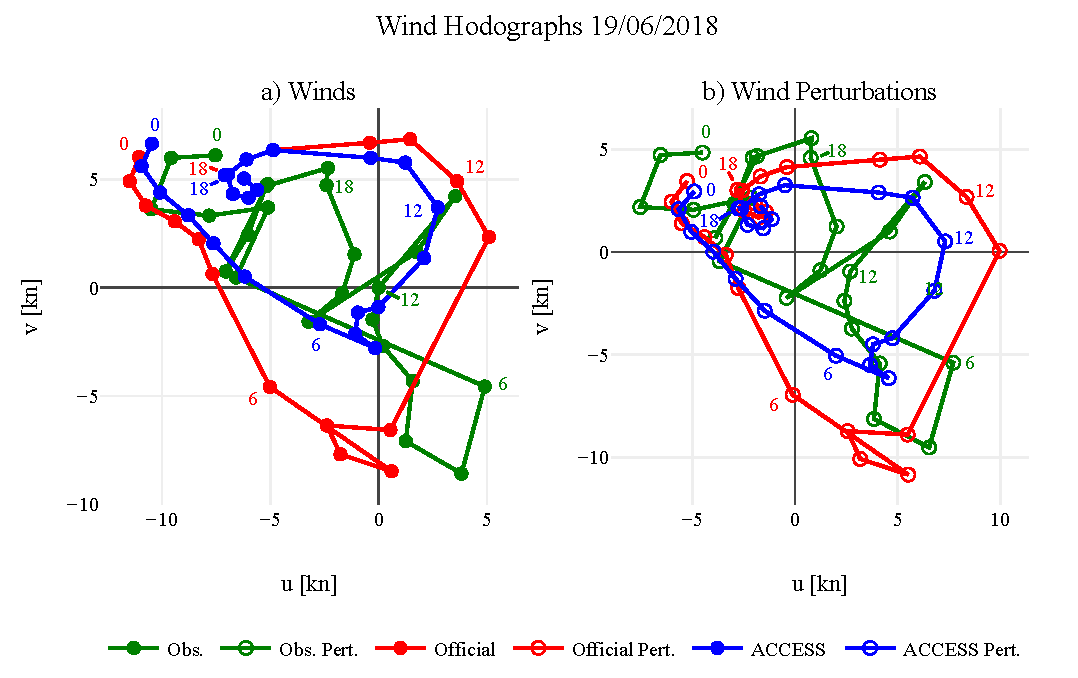
\includegraphics[width=0.90\textwidth]{daily_winds_darwin_AP.pdf}
\caption{TBA.}
\label{Fig:airport_wpi_access}
\end{figure}

\begin{figure}
\centering
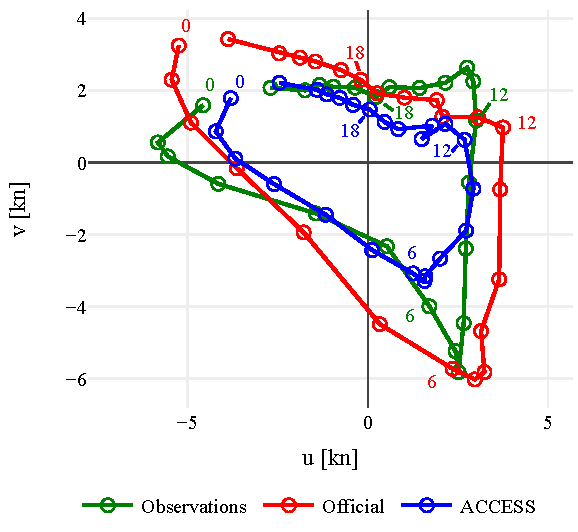
\includegraphics[keepaspectratio=true,width=0.55\textwidth]{clim_winds_austral_winter_ACCESS.pdf}
\caption{TBA.}
\label{Fig:airport_wpi_access}
\end{figure}

\begin{figure}
\centering
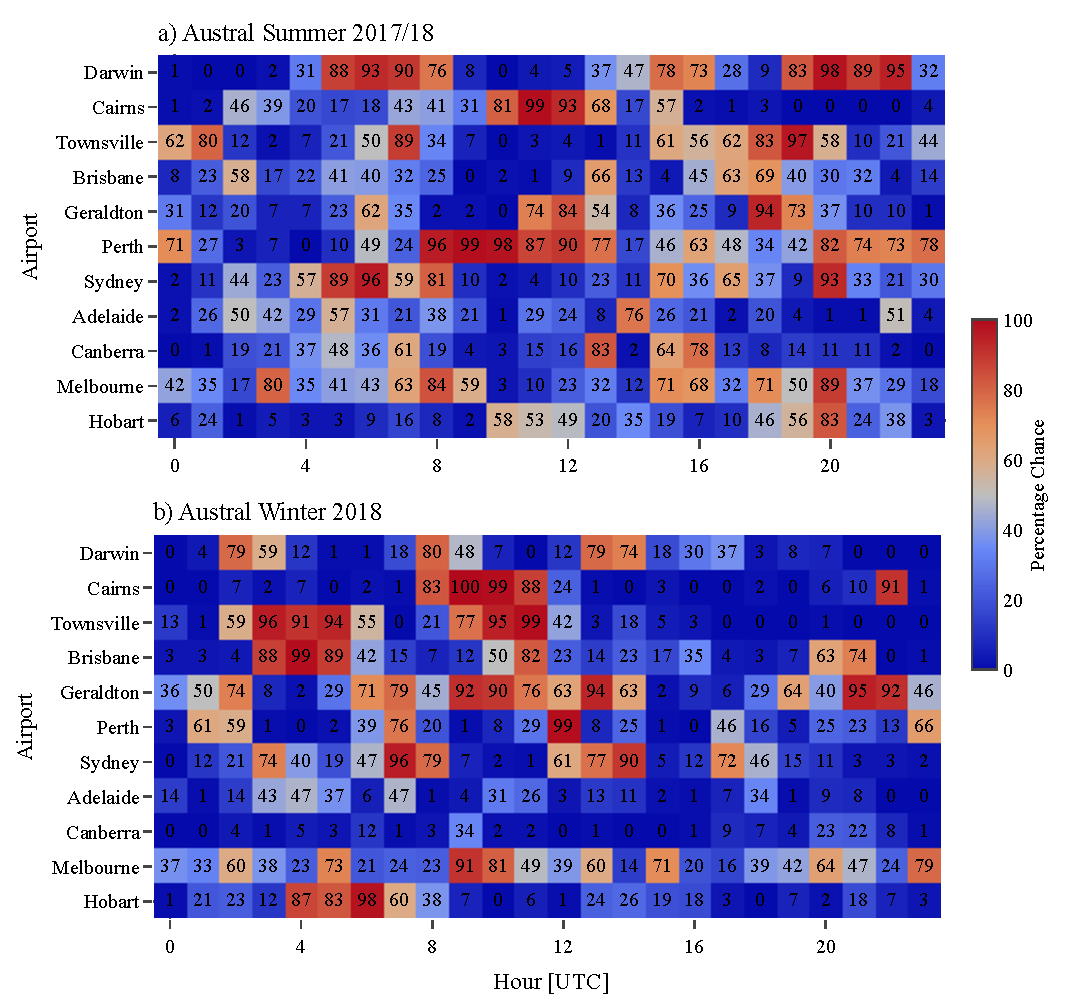
\includegraphics[keepaspectratio=true,width=0.90\textwidth]{airport_wpi_access.pdf}
\caption{Confidence that the Bureau's official forecasts of diurnal wind processes are more accurate than unedited ACCESS model guidance for a) the austral summer months (December, January, February) of 2017/18 and b) the austral winter months (June, July, August) of 2018, as measured by the WPI.}
\label{Fig:airport_wpi_access}
\end{figure}

\begin{figure}
\centering
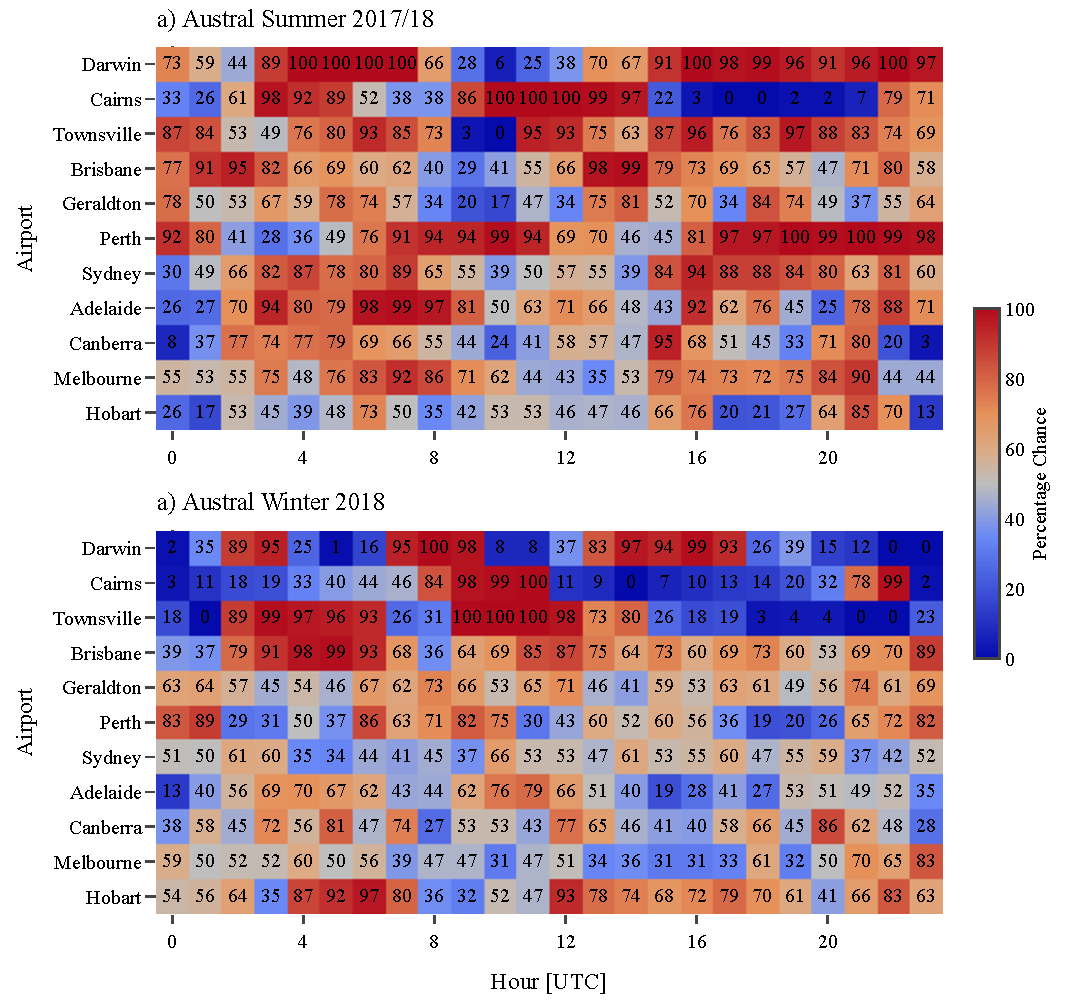
\includegraphics[keepaspectratio=true,width=0.90\textwidth]{airport_cwpi_access.pdf}
\caption{As in Fig.~\ref{Fig:airport_wpi_access}, but measured using the CWPI.}
\label{Fig:airport_cwpi_access}
\end{figure}

\begin{figure}
\centering
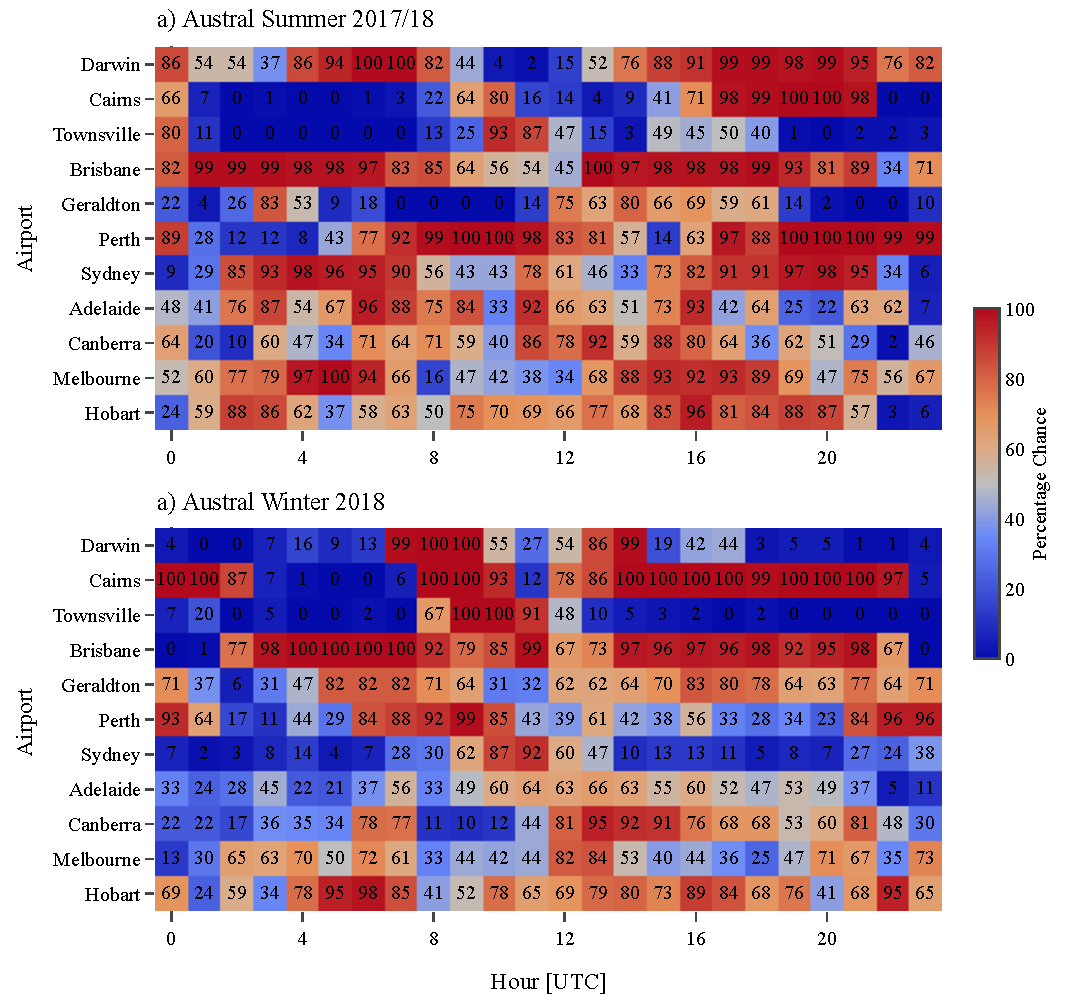
\includegraphics[keepaspectratio=true,width=0.90\textwidth]{airport_cwpi_ec_vs_access.pdf}
\caption{Confidence that diurnal wind processes are more accurate in ECMWF than in ACCESS using the CWPI. Tme periods as in Fig.~\ref{Fig:airport_wpi_access}.}
\label{Fig:airport_cwpi_access}
\end{figure}

\section{Conclusion}
In this report, a methodology for comparing the performance of Bureau forecasts of diurnal wind processes to unedited model guidance products has been developed and applied to a case study of the Darwin airport. The key results may be summarised as follows.
\begin{enumerate}
\item
During the dry season months of June, July and August 2017, the ECMWF sea-breeze is generally more accurate than that of the official forecast. However, during the wet season months of December, January and February 2017/18 this result is reversed, and the official forecast sea-breeze generally outperforms that of ECMWF. 
\item
In both seasons, boundary layer mixing processes are generally represented better in official forecasts than in ECMWF.
\item
In the dry season, the climatological wind perturbations of the official forecast generally outperform those of ECMWF between 13:00 and 16:00 UTC. This is due to ECMWF not capturing the magnitude of the south-easterly mean perturbations. 
\item
During the wet season, the climatological wind perturbations of the official forecast generally outperform those of ECMWF at 11:00 UTC. This is due to ECMWF underestimating the magnitude of the mean land-breeze perturbation.
\end{enumerate}    

There a number of ways that this work could be extended. The most pressing would probably be to investigate whether the results presented here change when a more operational definition of the sea breeze is used in place of the entirely perturbation based definition used here: this could be done using the method described in section \ref{methods}.

Following this, a nationwide study could be conducted focusing on the most operationally relevant locations of each state, for instance, airport stations. This should be done on a seasonal basis given that the examples considered here indicate results are seasonally dependent. The boundary layer mixing and sea-breeze editing techniques used by forecasters could then be collated and compared, with a view to standardising them across the country and optimising performance.

%%%%%%%%%%%%%%%%%%%%%%%%%%%%%%%%%%%%%%%%%%%%%%%%%%%%%%%%%%%%%%%%%%%%%%%%%%%%%%%%%%%%%%%%%%%%%%%%%%%%%%%%%%%%%%%%%%%%%%%%%%%%%%%%%%%%%%%%%%%%%%%%%
% Automagically insert a reference list

\bibliography{./Coastal_Winds.bib}

%%%%%%%%%%%%%%%%%%%%%%%%%%%%%%%%%%%%%%%%%%%%%%%%%%%%%%%%%%%%%%%%%%%%%%%%%%%%%%%%%%%%%%%%%%%%%%%%%%%%%%%%%%%%%%%%%%%%%%%%%%%%%%%%%%%%%%%%%%%%%%%%%

\end{document}
